\section{Modelo ARX}
\label{sec:arx}
%===============================================================================

O sistema real apresentado em (\ref{eq:system}) ser� identificado pelo modelo ARX onde
genericamente o modelo utilizado � como apresentado em (\ref{eq:generic_model}) e 
para o modelo ARX tem-se que apenas os polin�mios $A$ e $B$ s�o diferentes de 1. \cite{aguirre}

\begin{equation}
A(q, \theta)Y(t)=\frac{B(q, \theta)}{F(q, \theta)}U(t)+\frac{C(q, \theta)}{D(q, \theta)}e(t)
\label{eq:generic_model}
\end{equation}

Onde:

\begin{equation}
\begin{matrix}
A(q, \theta)=1+a_1 q^{-1}+a_2 q^{-2}+\cdots +a_{na} q^{-na}\\
B(q, \theta)=b_1 q^{-1}+b_2 q^{-2}+\cdots +b_{nb} q^{-nb}\\ 
C(q, \theta)=1+c_1 q^{-1}+c_2 q^{-2}+\cdots +c_{nc} q^{-nc}\\ 
D(q, \theta)=1+d_1 q^{-1}+d_2 q^{-2}+\cdots +d_{na} q^{-nd}\\ 
F(q, \theta)=1+f_1 q^{-1}+f_2 q^{-2}+\cdots +f_{nf} q^{-nf} 
\end{matrix}
\nonumber
\end{equation}

Desta forma o modelo ARX pode ser representado como em (\ref{eq:model_arg_g}). Para o
sistema apresentado em (\ref{eq:system}), o modelo ARX fica como em (\ref{eq:model_arx}).

\begin{equation}
A(q, \theta)Y(t)=B(q, \theta)U(t)+e(t)
\label{eq:model_arx_g}
\end{equation}

\begin{equation}
G(q, \theta )=\frac{a}{q-b}\;\;\;\;\;H(q, \theta)=\frac{q}{q-b}
\label{eq:model_arx}
\end{equation}

\begin{equation}
y(t)=G(q, \theta)r(t)+H(q, \theta)e(t)
\nonumber
\end{equation}

Onde $e(t)$ � ruido branco com m�dia zero.

Este modelo n�o consegue representar o sistema descrito em (\ref{eq:system}). 
Foi utilizado o script do matlab apresentado no Anexo (\ref{anx_arx_simul}) para 
simular as estimativas obtidas para os par�metros $a$ e $b$ deste modelo, o script
utiliza o m�todo dos m�nimos quadrados para estimar os par�metros.

O resultado da simula��o � apresentado na Figura (\ref{fig:arx}).

\begin{figure}[htbp]
	\center
	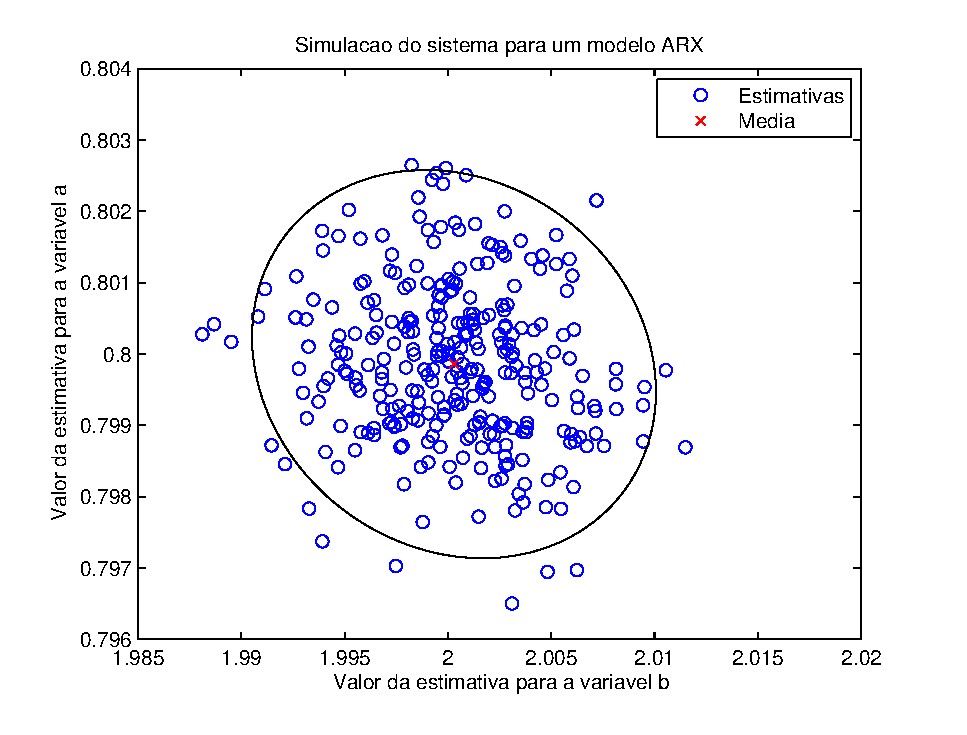
\includegraphics[width=0.98\columnwidth]{figures/arx.eps}
	\caption{Simula��o do sistema para uma entrada aleat�ria e utilizando o modelo ARX.}
	\label{fig:arx}
\end{figure}

A m�dia das estimativas obtidas para o sistema foi de $a=2.003$ e $b=0.7999$.

Aplicando na entrada do processo uma senoide de frequ�ncia $\pi /4$ obt�m-se a estimativa
como apresentado na Figura (\ref{fig:arx_sin_pi4}).

\begin{figure}[htbp]
	\center
	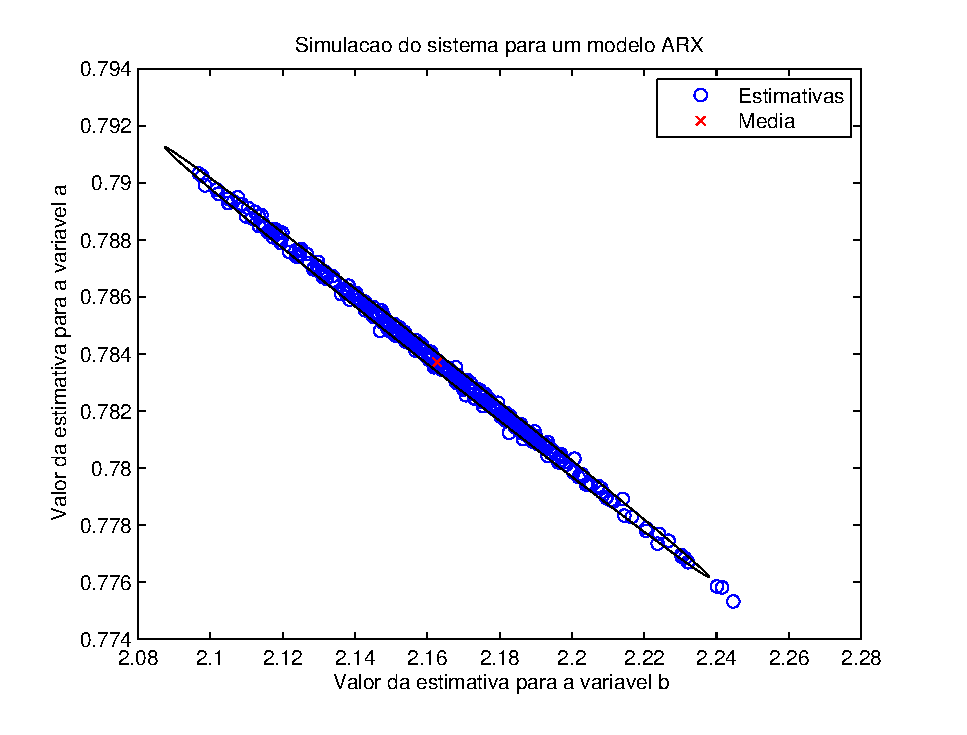
\includegraphics[width=0.98\columnwidth]{figures/arx_sin_pi4.eps}
	\caption{Simula��o do sistema para uma entrada $sin(\pi /4)$ e utilizando o modelo ARX.}
	\label{fig:arx_sin_pi4}
\end{figure}

A m�dia das estimativas obtidas para o sistema foi de $a=2.1627$ e $b=0.7837$.


Aplicando na entrada do processo uma senoide de frequ�ncia $\pi /20$ obt�m-se a estimativa
como apresentado na Figura (\ref{fig:arx_sin_pi20}).

\begin{figure}[htbp]
	\center
	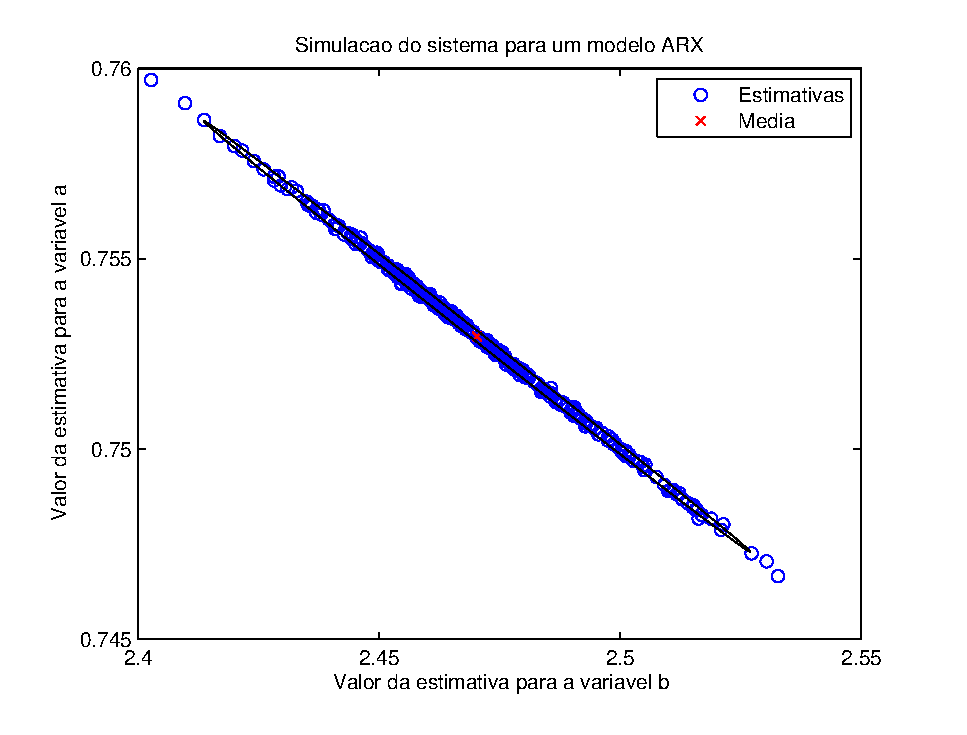
\includegraphics[width=0.98\columnwidth]{figures/arx_sin_pi20.eps}
	\caption{Simula��o do sistema para uma entrada $sin(\pi /20)$ e utilizando o modelo ARX.}
	\label{fig:arx_sin_pi20}
\end{figure}

A m�dia das estimativas obtidas para o sistema foi de $a=2.1687$ e $b=0.7831$.

Observa-se claramente que a estimativa est� polarizada, ou seja, a m�dia das estimativas 
n�o est� centrada nos valores reais dos par�metros. Isso de deve ao fato que o modelo utilizado
para a estimativa n�o consegue representar na totalidade o sistema original.

